\section{Inne programy}
\label{sec:inne_programy}

Podczas opracowywania oprogramowania,
które spełniać będzie obecne standardy ergonomii i intuicyjności,
warto zwrócić uwagę na inne popularne programy z odrębnych kategorii.
W szczególności będącym na darmowej licencji,
przez co są dostępne dla większej liczby użytkowników
i idealne do nauki danej dziedziny, której dotyczą.

\subsection{GIMP}
\label{subsec:gimp}

Podobnie jak Electric, GIMP jest oficjalnym pakietem GNU i również posiada otwarty kod źródłowy
oraz stosuje założenia wolnego oprogramowania~\cite{gimp_site}.
Jest dostępny na wiele platform, w tym na systemy Windows, Linux oraz macOS.
GIMP to program do edycji grafiki rastrowej.
Charakteryzuje się przejrzystym interfejsem graficznym oraz dużą ilością narzędzi,
gdzie każde z nich ma swój własny skrót klawiszowy, co znacznie ułatwia pracę w programie.
\indent Interfejs graficzny jest podzielony na trzy główne panele, nie licząc obszaru roboczego:

\begin{citemize}
    \item Górny panel menu programu -- dostępne opcje dla programu oraz dodatkowe opcje do modyfikacji edytowanego obrazu,
    \item Prawy panel -- zawiera przede wszystkim panel do zarządzania warstwami obrazu,
    ale również szereg innych opcji takich jak krzywe, desenie czy wybór pędzli
    \item Lewy panel narzędzi -- zawiera narzędzia do rysowania oraz modyfikacji obrazu oraz opcje tych narzędzi.
\end{citemize}

Widok okna programu GIMP przedstawiono na rys.~\ref{fig:gimp_okno}.
Dzięki zastosowaniu takiego interfejsu program jest przejrzysty dzięki zgrupowaniu konkretnych typów funkcjonalności,
co może mieć także zastosowanie w opracowywanym programie. \\
\indent Dzięki darmowemu dostępowi i szerokiej funkcjonalności,
GIMP został także wykorzystany do opracowania grafik do niniejszej pracy.

\begin{figure}[h]
    \centering
    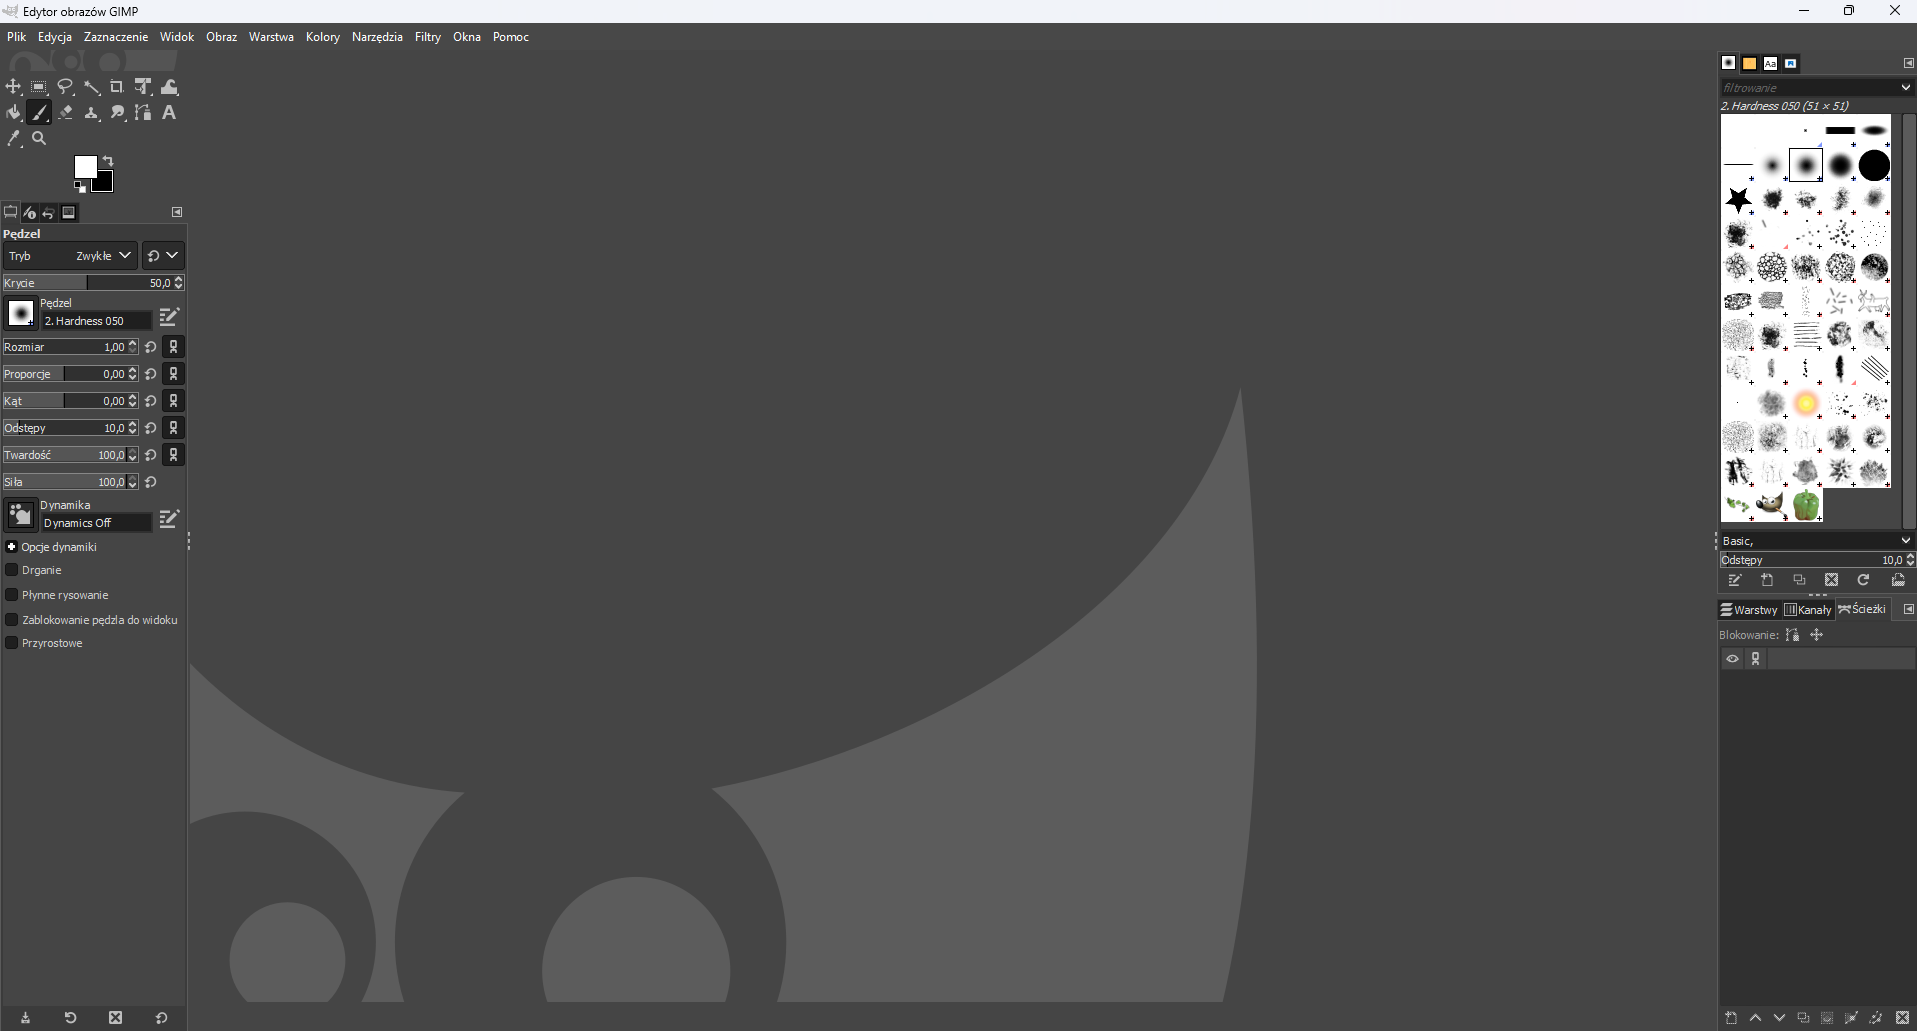
\includegraphics[width=.9\textwidth]{chapters/chapter2/img/gimp}
    \caption[Widok głównego okna programu GIMP.]{Widok głównego okna programu GIMP, źródło:~\cite{gimp_site}.}
    \label{fig:gimp_okno}
\end{figure}

\subsection{Blender}
\label{subsec:blender}

Program Blender jest kolejnym przykładem oprogramowania z otwartym kodem źródłowym na licencji GNU~\cite{blender_site}.
Wykorzystywany jest do tworzenia grafiki trójwymiarowej, animacji oraz efektów specjalnych.
Ze względu na rozbudowane możliwości oraz ilość narzędzi i funkcji,
zasadnicze znaczenie ma ergonomia i przejrzystość interfejsu, pokazanego na rys.~\ref{fig:blender_okno}.
Poza podobnymi jak w reszcie programów panelami górnym i prawym,
Blender wyróżnia się dolnym panelem z osią czasu do animacji, a także małym paskiem narzędzi w lewym górnym rogu okna,
co jest efektywnym sposobem pozwalającym na zaoszczędzenie miejsca na obszar roboczy,
gdy nie ma dużej liczby narzędzi do wykorzystania w danym momencie.
Podobne rozwiązanie może znaleźć zastosowanie w edytorze schematów.

\begin{figure}[h]
    \centering
    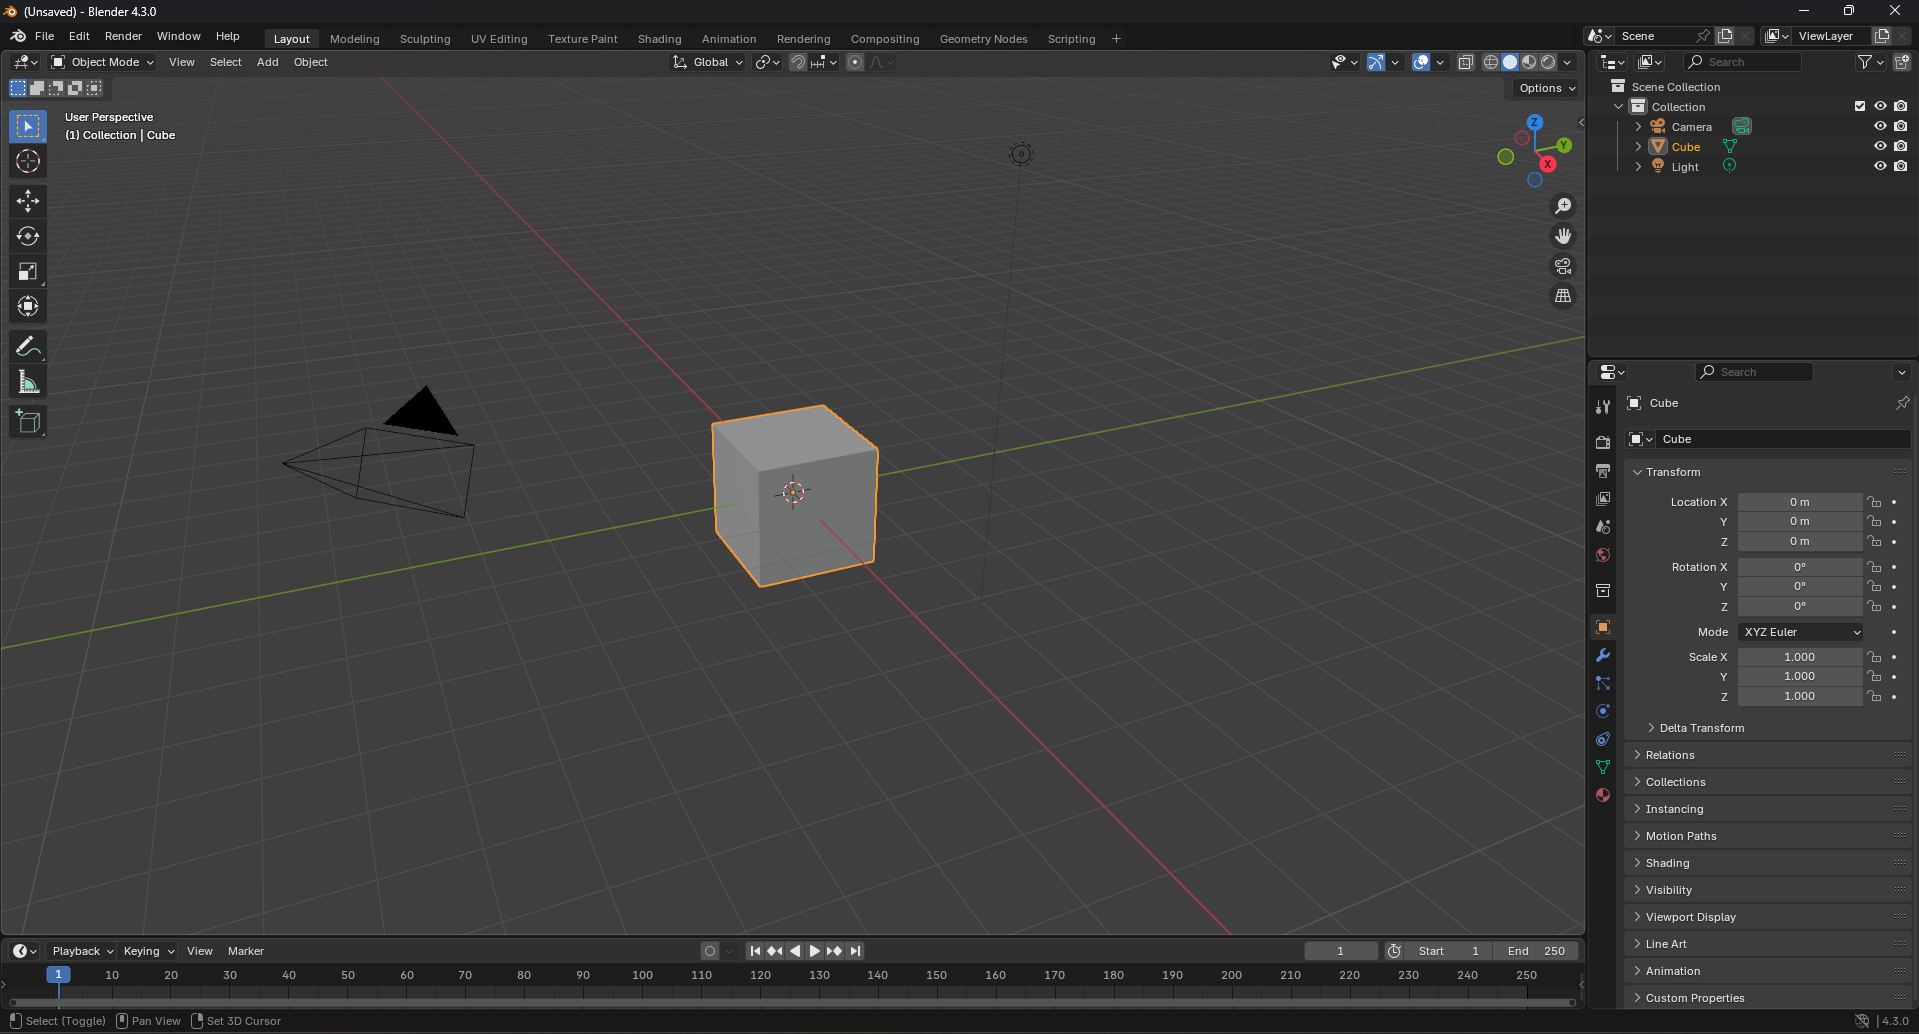
\includegraphics[width=.9\textwidth]{chapters/chapter2/img/blender}
    \caption[Widok głównego okna programu Blender.]{Widok głównego okna programu Blender, źródło:~\cite{blender_site}.}
    \label{fig:blender_okno}
\end{figure}
